\section*{Assignment 09: Scaling Strategy}
\addcontentsline{toc}{section}{Assignment 09: Scaling Strategy}

\subsection*{Phase one: proving product market fit}
The first phase runs within a single city so coordination stays manageable. I target sixty active students and twenty completed projects with satisfaction above four point five. These numbers come from the launch model in Assignment~02 and \citet{Choudary2016}'s suggestion to reach a minimum viable critical mass before expanding. Two anchor partners, ideally a municipal innovation unit and a trusted NGO network, lend legitimacy. The team structure includes a product lead, two engineers, a community manager, and part time mentor support. Weekly retrospectives log every friction point in a shared knowledge base so improvements remain evidence based.

\subsection*{Phase two: regional expansion}
Once the core loops hold, the second phase scales across the region. Onboarding flows become standardised templates, and the API described in Assignment~06 lets partners integrate without bespoke work. I introduce a three tier partner programme (community, certified, strategic) with criteria for response time, satisfaction, and contribution to fairness metrics. Targets grow to two hundred fifty active students, seventy five organisations, and time to first value under twelve hours. These thresholds align with \citet{HagiuWright2013}'s emphasis on balancing growth and quality. A partner success pod tracks retention and runs quarterly business reviews, borrowing rituals from enterprise SaaS but keeping tone informal.

\subsection*{Phase three: national network}
The final phase explores national or Nordic reach once unit economics stabilise. This step requires alliances with national agencies, expanded governance via an advisory board, and white label options for institutions that need their own branding. Success looks like five hundred projects per year, completion above ninety percent, and net revenue retention above one hundred ten percent. \citet{Srnicek2017} warns that scale without legitimacy invites backlash, so transparency reports and the inclusion council remain central.

\subsection*{Risk mitigation and decision gates}
Two risks dominate scaling plans: churn and quality drift. To manage churn I track retention per segment, run exit interviews, and maintain loyalty loops such as alumni storytelling events. To manage quality I enforce service level agreements on response times, automate match quality monitoring, and convene a community board when satisfaction dips below four point four for two consecutive months. If that happens, new partner onboarding pauses until remediation steps pass a board vote. Figure~\ref{fig:scaling-dashboard} visualises the dashboard that would watch these signals.

\begin{figure}[H]
  \centering
  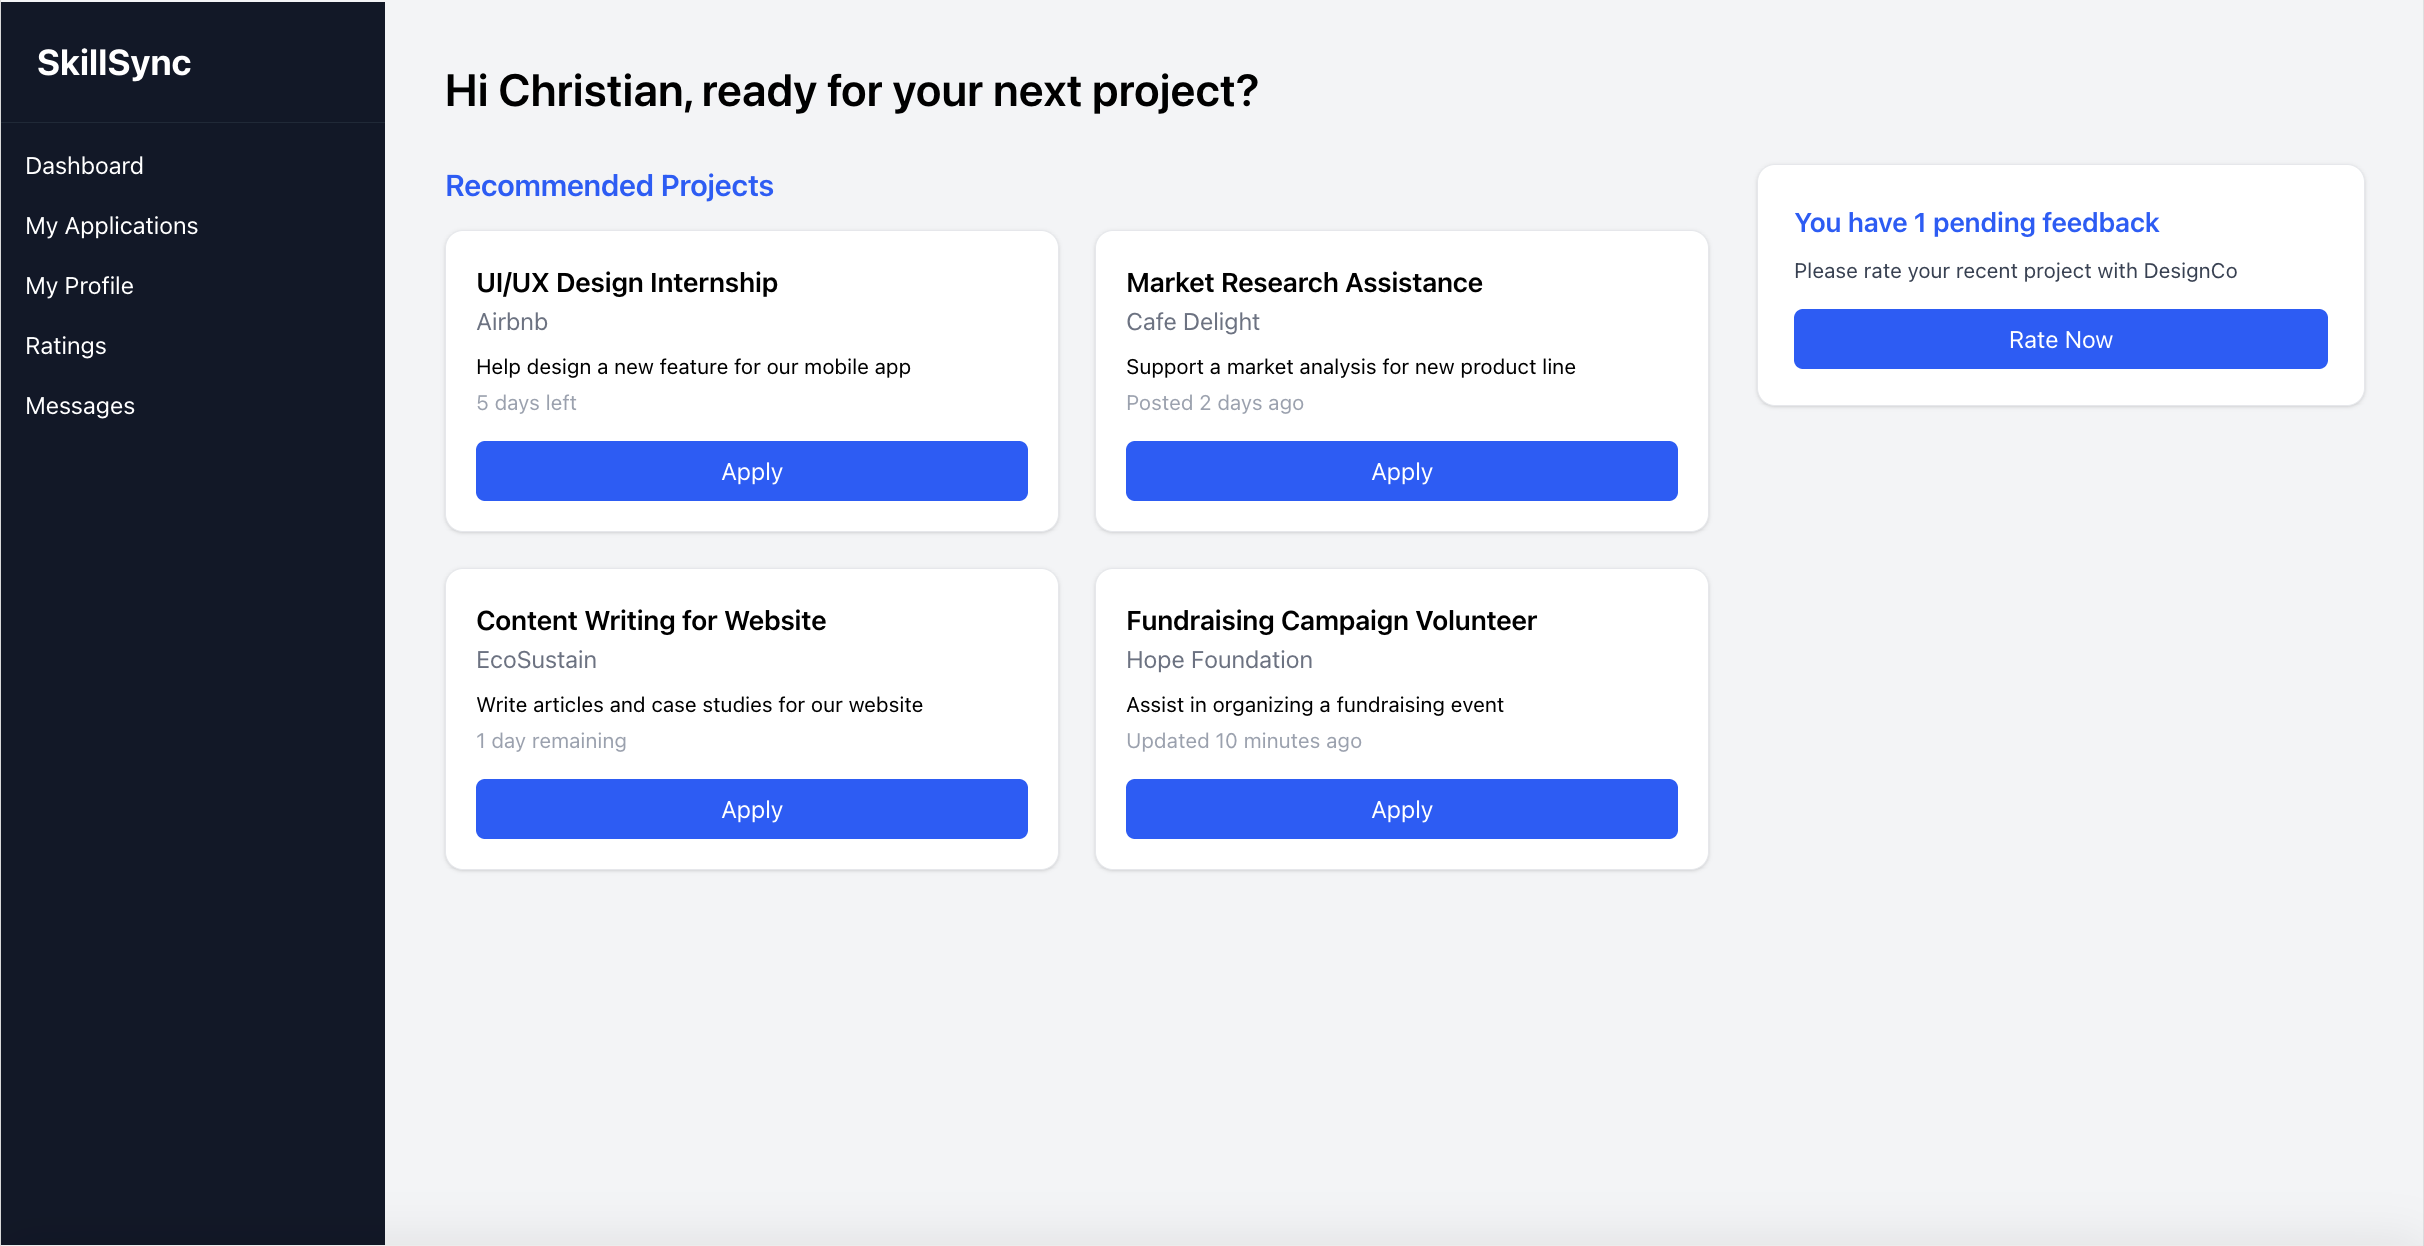
\includegraphics[width=0.75\linewidth]{figures/Student-Dashboard.png}
  \caption{Adoption dashboard mock up tracking activation against partner enablement.}
  \label{fig:scaling-dashboard}
\end{figure}

\subsection*{Scenario modelling}
To test resilience I built a Google Sheets simulation tracking activation rate, moderation load, partner velocity, and revenue per project. The model estimates staff needs per one thousand active users and includes a pause rule: if satisfaction stays below four point four for eight weeks, growth spending freezes. I also modelled a downside case where retention drops five points; it lowers annual revenue by roughly nine million DKK and delays break even by twelve months, so the playbook includes a cost reduction plan that prioritises core trust features. These exercises apply \citet{Lecture12}'s recommendation to treat scaling as a system design problem rather than a marketing stunt.
